\section{Motivation --- Cloud-centric Usage Management}

% Outline
% I. Frame the problem (use the AF proposal for this)
% II. Outline current solutions from UCDMO using guards
% III. Discuss problems (use pro/con list)
% IV. Frame specific challenges using slides II, III

\begin{frame}[t]
\frametitle{The Problems --- Customer Perspectives}
Current policy-centric systems are being forced to move to cloud environments and build much more open systems.  Usage management is a key problem in this domain --- information needs to be delivered to those who need it as soon as possible:
\newline
\newline
"...It is imperative to  effectively exchange information among components, Federal agencies, coalition partners, foreign governments and international organizations as a critical element of our efforts to defend the nation and execute national strategy..."\cite{proposal:info-sharing-strategy}
\newline
\begin{footnotesize}\textit{--- DoD Information Sharing Strategy}\end{footnotesize}
\newline
\newline
"...The CIO of the National Security Agency is focusing on IT architecture and a cloud-centric approach to sharing information..."\cite{proposal:nsa-cloud}
\newline
\begin{footnotesize}\textit{--- Informationweek}\end{footnotesize}
\end{frame}

\begin{frame}[t]
\frametitle{The Problem --- Characteristics}
Cloud systems may save money, provide more flexibility, but they also \cite{proposal:privacy-security-trust-cloud}:
\begin{itemize}
\item<2-> \textit{Are Not Private} --- User data control in SaaS is lacking, causing policy concerns for agencies; Data owners have no technical control over secondary use; providers may use offshore development; data can be routed across sensitive countries or secondarily stored on CDNs; data privacy on bankruptcy is ill-defined
\item<3-> \textit{Are Less Secure} --- Controlling data access, data may not be wiped in all XaaS scenarios, availability/backup leads to possible data proliferation, lack of standardization in intercloud communication and data transfer, multi-tenancy and side-channel attacks, difficult logging/auditing
\item<4-> \textit{Cannot Be Trusted} --- Trust relationships, consumer trust
\end{itemize}
\end{frame}

\begin{frame}[t]
\frametitle{Current Solutions}
How are these problems being addressed by impacted organizations?
\newline
\newline
\pause
They're just starting to be actively addressed and are an open research question \cite{proposal:assured-info-sharing}.
\newline
\newline
Cross-domain architectures are currently the standard for monitoring and information dissemination in an effort lead by the \textit{Unified Cross Domain Management Office}, associated with the Department of Defense (DoD) and the National Security Agency (NSA).
\end{frame}

\begin{frame}[t]
\frametitle{Current Solutions --- NSA}
Legacy cross-domain notional architecture \cite{proposal:nsa-arch}
\begin{figure}[!t]
\centering
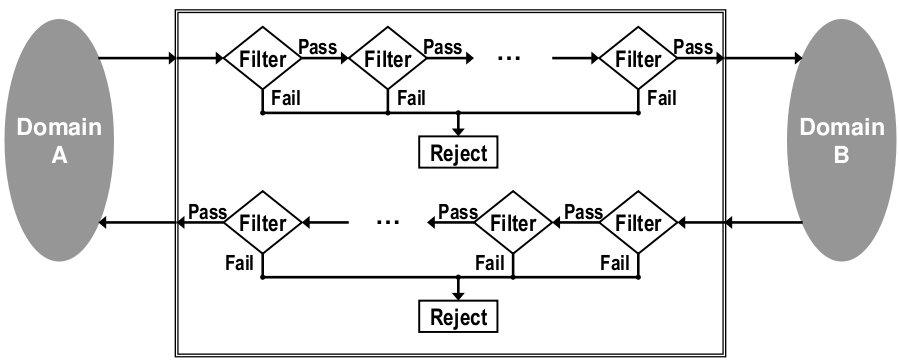
\includegraphics[width=3.4in]{nsa-legacy-arch}
\caption{NSA Legacy Model}
\label{fig:model:conceptual-model}
\end{figure}

\textit{Domain A} --- Private cloud managed by the Air Force
\newline
\textit{Domain B} --- A public operational network
\end{frame}

\begin{frame}[t]
\frametitle{Current Solutions --- NSA (SoA)}
Future cross-domain notional architecture \cite{proposal:nsa-arch}
\begin{figure}[!t]
\centering
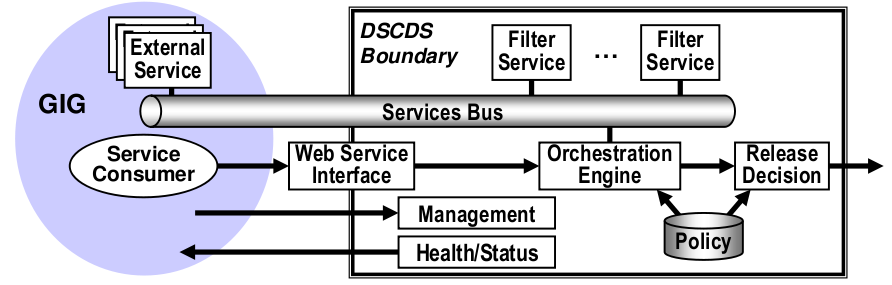
\includegraphics[width=3.4in]{nsa-arch}
\caption{NSA Service-Oriented Model}
\label{fig:model:conceptual-model}
\end{figure}

\textit{GiG} --- Global Information Grid; a large public cloud operated by the DoD
\newline
\textit{DSCDS} --- Distributed Service-oriented Cross Domain Solution
\end{frame}

\begin{frame}[t]
\frametitle{Current Solutions --- Raytheon}
Raytheon's notional architecture supporting cross-domain information flow \cite{proposal:raytheon-arch}:
\begin{figure}[!t]
\centering
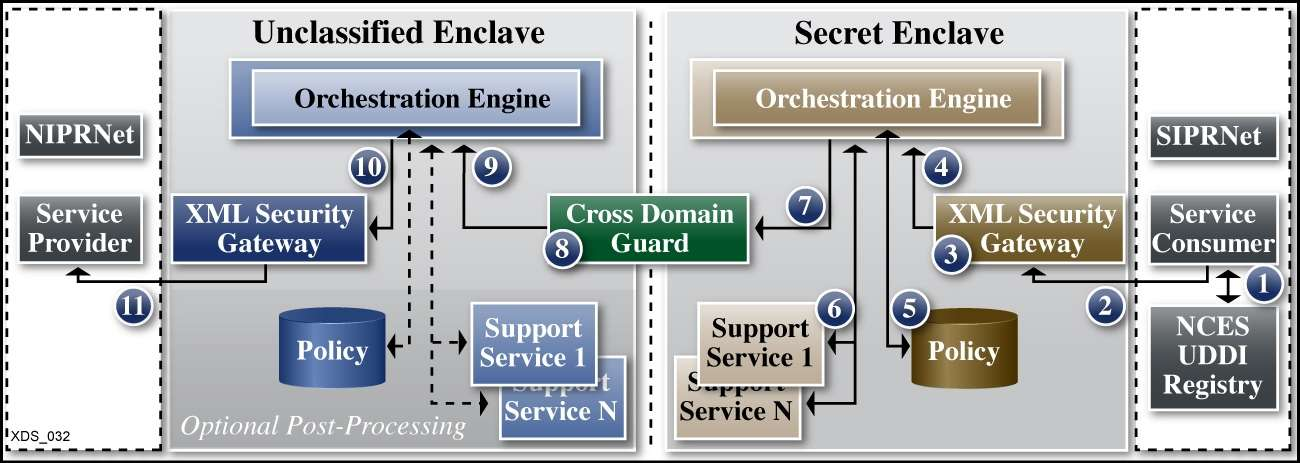
\includegraphics[width=3.4in]{raytheon-arch}
\caption{Raytheon Model}
\label{fig:model:conceptual-model}
\end{figure}

\textit{...still uses a single perimeter guard...}
\end{frame}

\begin{frame}[t]
\frametitle{Current Solutions --- BAH}
Booz|Allen|Hamilton presented a service-centric cross domain solution in 2009 \cite{proposal:bah-arch}:
\begin{figure}[!t]
\centering
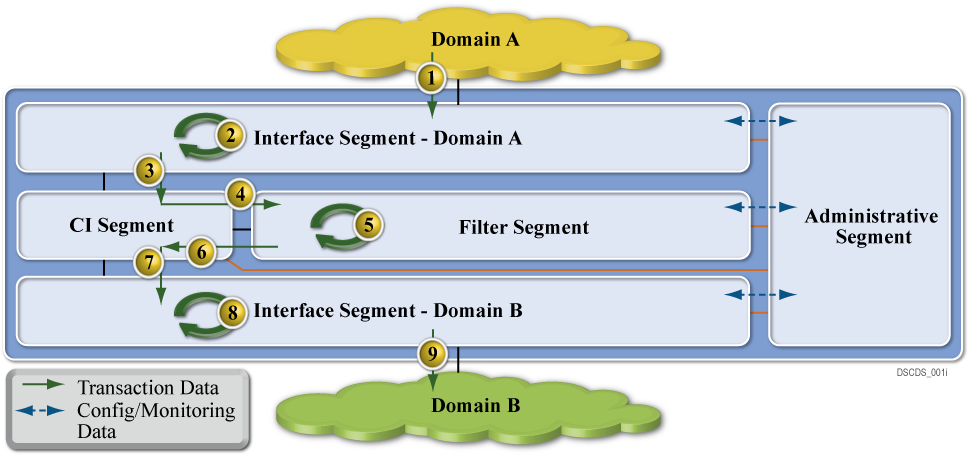
\includegraphics[width=3.4in]{bah-arch}
\caption{Booz|Allen|Hamilton Model}
\label{fig:model:conceptual-model}
\end{figure}
\textit{...still uses a single perimeter guard (called a filter segment)...}
\end{frame}

\begin{frame}[t]
\frametitle{Future Solution}
Organizations are falling back on what they know in the scope of new problems.
\begin{figure}[!t]
\centering
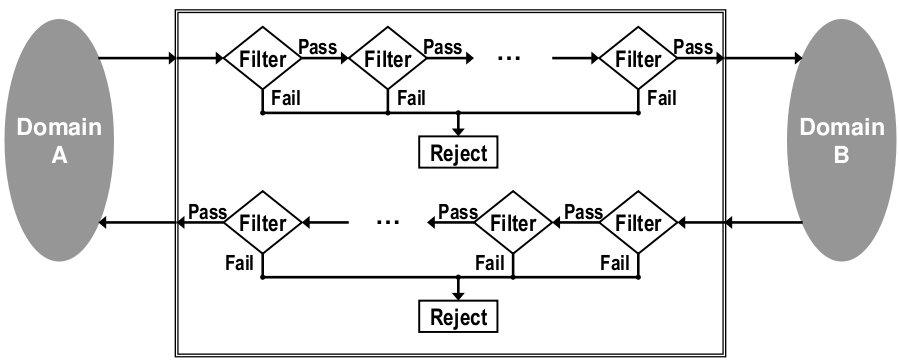
\includegraphics[width=3.4in]{nsa-legacy-arch}
\caption{NSA Legacy Model}
\label{fig:model:conceptual-model}
\end{figure}
Even though we know they don't work \cite{proposal:ron-ross}.
\end{frame}

%overlay:
%- Policy into network fabric
%- Multiple compartments on same physical network
%- Network can integrate cloud components securely
%- Provides security in depth
%
%traditional/guard:
%- Policy centralized single points of failure
%- Each physical network can only be at one compartment level
%- Use is tied to the physical network; no cloud integration possible
%- Boundary security only 
\begin{frame}
\frametitle{Characteristics of Current Solutions}
\begin{itemize}
\item<2-> \textit{Centralized Policy} --- They use centralized policy injection into communication flow.  Note that in each sample model, policy is \textit{only} evaluated at guard points.
\item<3-> \textit{Physical to Compartment Mapping} --- In each of these cases, users are only allowed to exchange one type of information per domain.  The physical domain systems are locked (by operational policy) to a single classification level limit.  Users cannot, for example, have \emph{Top Secret} material on a network accredited for \emph{Secret} material.
\item<4-> \textit{Perimeter Protection} --- The use of a single policy enforcement point at domain interconnects supplies a crunchy exterior to the creamy interior data filling.
\end{itemize}
\end{frame}

\begin{frame}
\frametitle{What's Wrong with Current Solutions?}
\begin{itemize}
\item<2-> \textit{Centralized Policy} --- A centralized policy enforcement system simplifies infrastructural attacks.  Adversaries know exactly where to focus efforts to compromise policy enforcement, lowering overall system trustworthiness and reliability. 
\item<3-> \textit{Physical to Compartment Mapping} --- The traditional model for multi-level security, enforced in this scheme, is that the network is classified at the level of the most sensitive data that transits it.  Ergo, those that have clearances at a level to view sensitive data are unable to view that data generally without extensive swivel-chair integration.
\item<4-> \textit{Perimeter Protection} --- Perimeter protection is a necessary but not sufficient security approach.  By itself, it doesn't work \cite{proposal:ron-ross}.
\end{itemize}
\end{frame}

\begin{frame}
\frametitle{Characteristics of Future Solutions}
\begin{itemize}
\item<2-> \textit{Decentralized Policy} --- Policy management is decentralized and integrated within the fabric of the system.  The system is both more secure and resilient as a result, better able to control information and operate under stressful conditions.
\item<3-> \textit{Infrastructure Reuse} --- Multi-tenancy can lower costs and increase reliability and is furthermore a common attribute of cloud systems.  An appropriately secured system facilitates integration of computing resources into multi-tenant environments.
\end{itemize}
\end{frame}

\begin{frame}
\frametitle{Characteristics of Future Solutions}
\begin{itemize}
\item<2-> \textit{Cloud Integration} --- The ability to handle multi-tenant environments and to reliably secure both data at rest and data in motion leads to computational environments deployable in cloud systems.
\item<3-> \textit{Security in Depth} --- Systems must operate under \textit{all} conditions, including when they are under attack or compromise \cite{proposal:ron-ross}.  Ergo, they must provide protection to sensitive data in depth.
\end{itemize}
\end{frame}
